\chapter{Multiple Integrals}
\setcounter{exercisecounter}{0}

\setcounter{thmcounter}{0}
\section{Introduction}

By this point, you should have noted that the geometry of $\mathbb{R}^n$ is intimately connected to calculus. Partial derivatives and tangent planes go hand in hand. However, if there's anything to take away from your first calculus course is that derivatives also go hand in hand with integrals. So you have every right to ask ``What does it mean to do integrals in higher-dimensions?'' This chapter will focus on developing the core concepts that surround this question. We will make sense of integrals in $2$ and $3$ dimensions by generalizing our intuition for the $1\text{D}$ case. We will see how --- in certain situations --- we can convert double and triple integrals into a simple iteration of singular integrals. Finally, we will derive the multidimensional version of the change of variables formula. Along the way, various applications to other disciplines will be presented, and you are encouraged to test your understanding via the exercises in each section. 

To start our discussion, let's remind ourselves of what it means to integrate a real-valued function $f(x)$ along some interval $I = \{x\in \mathbb{R}: \ a \le x \le b\}$,
\begin{equation}
    \int_a^b f(x) \ \mathrm{d}x
\end{equation}
Intuitively, we interpret this as the signed area determined by $f(x)$ when $x\in I$. But how do we compute this area, in general? A good strategy is to partition the interval into very small chunks that are easier to deal with, and then add up their individual contributions to the integral. To that effect, let's partition the interval $I$ into a sequence of intervals $I_1, I_2, \cdots, I_n$ according to a sequence of points $a = x_0 < x_1 < \cdots < x_{n-1} < x_n = b $. In other words, take $I_k = [x_{k-1}, x_k]$. This procedure is demonstrated in Figure \ref{fig:riemman_sum}. Now, take a representative point $\tilde{x}_k \in I_k $ from each interval. It doesn't matter what this point is exactly, as we are assuming the intervals are small enough such that the function doesn't change very much within each interval. The signed area of $f$ on each of the $I_k$ is approximately $f(\tilde{x}_k) (x_k - x_{k-1})$. Thus, since $I = I_1 \cup I_2 \cdots \cup I_n$, we can approximate the integral as follows:
\begin{equation}
    \int_a^b f(x) \ \mathrm{d}x \approx \sum_{k=1}^n f(\tilde{x}_k) (x_k - x_{k-1})
\end{equation}
The right-hand side is a \textit{Riemman sum}, as you learned in your calculus course. We can  measure the accuracy of our approximation by the largest interval width $\sigma = \max_k\{ x_k - x_{k-1}\}$. Then, we define\footnote{Note that the Riemman sum is not a function of $\sigma$, so there are some subtleties in how we define this limit. You don't need to worry about them for now. You just need to note that the Riemman sum is definitely constrained by $\sigma$. } the \textit{Riemman integral} to be:
\begin{equation}
    \label{eq:riemman_integral}
    \int_a^b f(x) \ \mathrm{d}x \defeq \lim_{\sigma \rightarrow 0} \sum_{k=1}^n f(\tilde{x}_k) (x_k - x_{k-1})
\end{equation}
\begin{figure}
    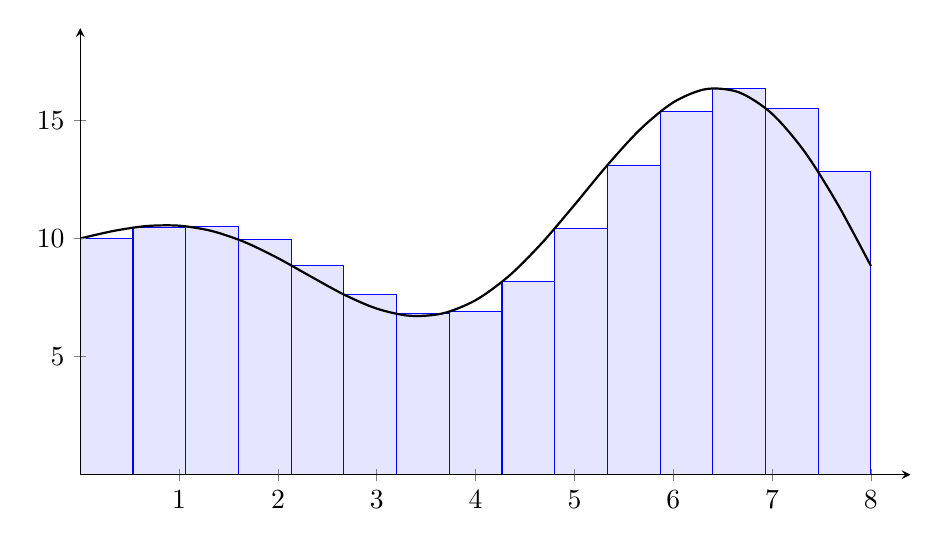
\begin{tikzpicture}
        \def\func{x * cos(deg(x))+10}
        \begin{axis}[
            xtick={0,...,10},ytick={5,10,15,20,25},
            width=\textwidth, y=0.3cm, xmax=8.4,ymax=18.9,ymin=0,xmin=0,
            enlargelimits=true,
            axis lines=middle,
            clip=false,
            domain=0:8,
            axis on top
            ]
        %\addplot [draw=red,fill=red!10,const plot mark left, samples=6]
        %    {1+x^2}\closedcycle;
        \addplot [draw=blue, fill=blue!10, ybar interval, samples=16]
            {\func}\closedcycle;
        \addplot[smooth, thick,domain=0:8]{\func};
        \end{axis}
    \end{tikzpicture}
    \caption{In this plot, we took $\tilde{x}_k = x_{k-1}$.}
    \label{fig:riemman_sum}
\end{figure}

We can use this definition to calculate various quantities of relevance in science. For example, imagine someone gives you a rod of length $L$. The rod is made of an insulating material, and it is charged with a linear charge density $\rho(x)$, for $x \in [0, L]$. The total charge $Q$ stored in the rod is given by the integral:
\begin{equation}
    Q = \int_0^L \rho(x) \ \mathrm{d} x
\end{equation}
In terms of the Riemman sum, we visualize the rod as a set of tiny point masses with charge $\rho(\tilde{x}_k) (x_k - x_{k-1})$ glued together, each contributing a small amount to the total charge of the rod. But what if someone gave us a charged sheet instead? Suppose you are also given an area charge density $\rho(x,y)$, how would you calculate the total charge of this sheet? Well, there's no reason why the divide and conquer strategy shouldn't work here as well. Let's get to work!

Suppose the sheet is represented by a region $R \in \mathbb{R}^2$. We will focus on the rectangle $A = [x_0, x_m] \times [y_0, y_n]$ that ``bounds'' the region. It can be subdivided into a grid of smaller rectangles obtained from subdividing the intervals $[x_0, x_m]$ and $[y_0, y_n]$ as we did with the $1\text{D}$ case. For a visual aid, check Figure \ref{fig:2driemman_sum}. We want to add up the contributions just from the rectangles that lie inside the region $R$, so we need to evaluate $\rho$ at a select group of rectangles while avoiding the others. This is complicated in general, so as a computational trick, we will define an auxiliary function $\tilde{\rho}(x,y)$ that agrees with $\rho(x,y)$ inside $R$, but is zero outside $R$.\footnote{We know that $\rho(x,y)$ is well-defined in $R$, but we have no idea what it does outside $R$. Maybe it describes the charge density of another object, or maybe it's not defined there. In the general case, we need to be careful.} Then, choose points $(\tilde{x}_i, \tilde{y}_j)$ inside the $(i,j)\text{-rectangle}$. By analogy with our intuition for the single integral, the small amount of charge contributed from that rectangle is $\tilde{\rho}(\tilde{x}_i, \tilde{y}_j)\Delta x_i \Delta y_j$ (where $\Delta x_i = x_i - x_{i-1}$ and $\Delta y_j = y_j - y_{j-1}$). Thus, we can approximate the total charge $Q$ of the charged sheet by
\begin{equation}
    Q \approx \sum_{i=1}^{m} \sum_{j=1}^{n} \tilde{\rho}(\tilde{x}_i, \tilde{y}_j)\Delta x_i \Delta y_j
\end{equation}
\begin{figure}
    \centering
    \begin{tikzpicture}
        \def\func{x * cos(deg(x))+10}
        \begin{axis}[
            xtick={0,0.5,...,10},ytick={1,1.5,...,5},
            width=\textwidth, height=0.5 \textwidth, 
            xmax=9.4, ymax=5.4, ymin=1, xmin=1,
            enlargelimits=false,
            axis lines=middle,
            clip=true,
            domain=0:10,
            axis on top,
            axis equal image,
            grid = major
            ]
            \draw [thick, solid] (axis cs: 2,2) rectangle (axis cs: 8,5);
            \addplot [name path=A, smooth, domain=2:8] {-0.2*(x-5)^2+5};
            \addplot [name path=B] coordinates {(2, 3.2) (3,2) (5,3) (7,2) (8, 3.2)};
            \addplot [blue!10] fill between [of=A and B];
            \node at (axis cs:5,4) [anchor=center, color=blue, font=\Large] {$R$};
            \node[pin={below left:$A$}] at (axis cs:2,5) {};
        \end{axis}
    \end{tikzpicture}
    \caption{A set of small rectangles with a larger rectangle $A$ bounding the region $R$. }
    \label{fig:2driemman_sum}
\end{figure}
At this point, you must be anticipating that to get the exact answer we just need to take the limit as $\sigma_x = \max_i \{\Delta x_i\}$ and $\sigma_y = \max_j \{\Delta y_j\}$ go to zero, like we did for the $1\text{D}$ case. However, just as we needed to be careful when taking limits in $\mathbb{R}^2$ (recall that the limit can't depend on the path taken towards the limit point), we need to be careful here. If we take the limit as $\sigma_x \rightarrow 0$ first, then $\Delta x_i \rightarrow 0$ and we end up with a bunch of rectangles of finite height and zero width. That amounts to adding zeros and our strategy fails. Similarly, it's not possible to take the limit as $\sigma_y \rightarrow 0$ first. We want both dimensions of the rectangles to become small ``at the same time.'' A reasonable way of doing this is to declare that the largest dimension $\sigma = \max \{\sigma_x, \sigma_y \}$ of the rectangles must go to zero. Definition \ref{def:double_integral} is as precise as we can make this statement in this course. When the limit exists, $f$ is said to be \textit{integrable} over the region $R$. Note that being integrable depends on \textit{both} $f$ and $R$. Under different formalizations of how one actually takes this limit, the same function might be classified as integrable or not. Well-behaved functions might not be integrable if the region $R$ is poorly-behaved, and vice versa. These pathological cases are not of interest right now, so from now on we will assume both $R$ and $f$ are ``nice enough.'' In particular, if $R$ is the union of finitely many \hyperref[def:elementary_regions]{elementary regions} (as defined in the next section), then any continuous function $f$ is integrable regardless of how you formally perform the limiting process.

% limits of nets 

\section{Double Integrals}

Based on the preceding discussion, we take Definition \ref{def:double_integral} to capture the basic notion of integrating over a region in $\mathbb{R}^2$. Note that the double integral is a fundamentally two-dimensional concept: the symbol $\iint$ is there just as an analogy to the one-dimensional case. As of right now, we have no idea how to compute double integrals for any reasonable function. A priori, you shouldn't look at them as two single integrals nested together. But it seems reasonable that they \textit{should} be related to single integrals in some way. The results later in this section will indeed establish that this intuition is correct, providing a computational method to deal with multidimensional integrals. Before we engage with such powerful tools, we need first to look at these objects from a geometrical perspective.

\begin{adefinition}{Double Integral}{double_integral}
    If $R \subseteq \mathbb{R}^2$ is a finite region and $f: R \rightarrow \mathbb{R}$ is a function, then the double integral of $f$ over the region $R$, is given by the following limit, when it exists:
    
    \begin{equation*}
        \iint_R f(x,y) \ \mathrm{d} A \defeq \lim_{\sigma \rightarrow 0} \sum_{i=1}^{m} \sum_{j=1}^{n} \tilde{f}(\tilde{x}_i, \tilde{y}_j)\Delta x_i \Delta y_j
    \end{equation*}
    
\end{adefinition}

What general feature of integral is illustrated by Figure \ref{fig:riemman_sum}? For each $x$, $f(x)$ is the height of the graph of the $f$ at that point, so when we multiply it by the length of a thin rectangle in the \hyperref[eq:riemman_integral]{Riemman sum} and add all pieces together, we get the signed area determined by $f(x)$ on the interval. How does this generalize? Assume now $f(x,y)$ is a function $R\rightarrow \mathbb{R}$. For each tiny rectangle at $(x,y)$, we are multiplying the value of a function $f(x,y)$, which is the height of the graph of $f$ at $(x,y)$. Thus, when we look at the graph of a two-variable function, its double integral over some region $R$ is just the net volume covered by $f(x,y)$ in that region. Let's take this opportunity to do some programming and visualize things. Assume $f(x,y) = \sqrt{1-x^2-y^2}$, defined on the unit disk centered at the origin. $D$. We will compute an approximation for $\iint_D f(x,y) \ \mathrm{d} A$ using Python.

\begin{figure}[h!]
    \centering
    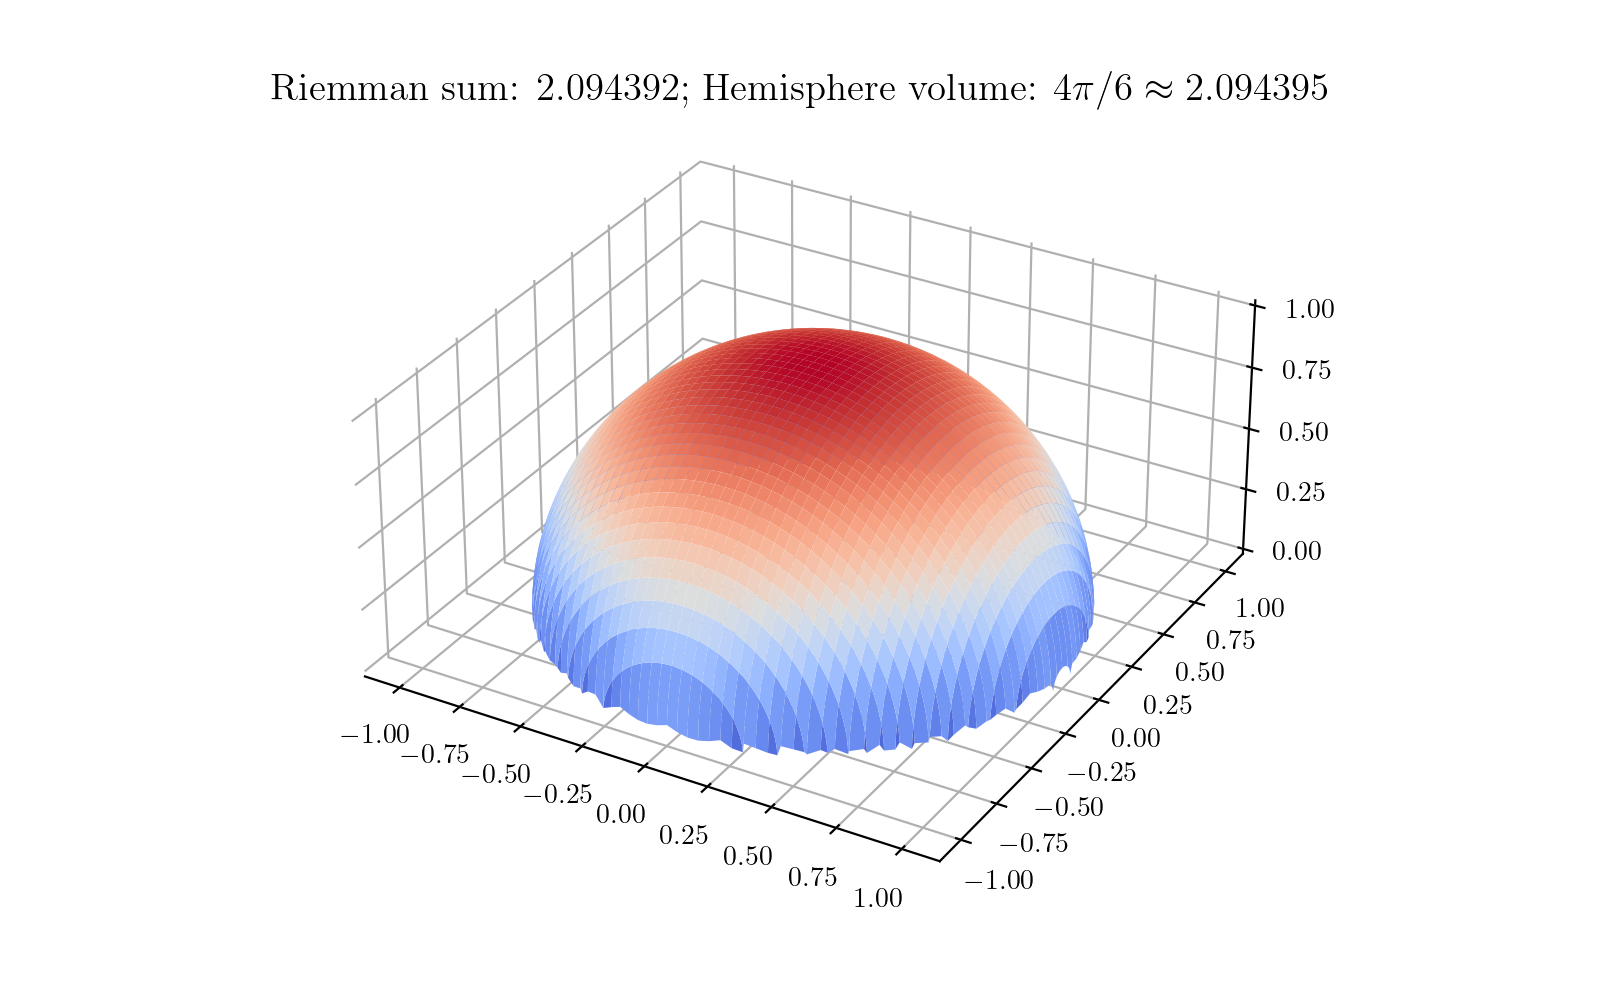
\includegraphics[width=\textwidth]{second_quarter/double_integral.png}
    \caption{The hemisphere surface $z = \sqrt{1-x^2-y^2}$.}
    \label{fig:hemisphere}
\end{figure}

Using the code in the next page, we calculated the volume enclosed by the hemisphere surface and the $xy$-plane in Figure \ref{fig:hemisphere} to be $2.094392$. From elementary geometry, we know the answer should be $4 \pi /6 \approx 2.094395$. The error comes, of course, from the fact that the Riemman sum is just an approximation, not the exact answer. As we increase the number of sampling points (i.e. make the rectangles smaller), these errors go away and the sum gets closer to the correct value, which is the integral. Our task now will be to learn how to get the exact value using some additional facts about double integrals.

\pagebreak

\begin{lstlisting}[language=Python]
import numpy as np
import matplotlib.pyplot as plt
from matplotlib import cm
# Use a 3d projection
fig, ax = plt.subplots( subplot_kw={"projection": "3d"}, 
                        figsize=(8,5), dpi=200)

# Increasing the number of sampling points will reduce
# the jagged edges around the equator and increasing accuracy
# of the integration.
sampling_points = np.linspace(-1, 1, 1000)

# X and Y are matrices containing the x and y coordinates of the sampling points
X, Y = np.meshgrid(sampling_points, sampling_points, indexing='ij')

# For each coordinate, we need not to sample at the last point as it
# belongs to the next interval [1, 1+delta]
Z = np.sqrt(1- X[:-1,:-1]*X[:-1,:-1] - Y[:-1,:-1]*Y[:-1,:-1])

surface = ax.plot_surface( X[:-1,:-1], Y[:-1,:-1], Z,
                           cmap=cm.coolwarm, linewidth=0, 
                           antialiased=True)

ax.set_xticks([-1 + 0.25 *n for n in range(9)])
ax.set_yticks([-1 + 0.25 *n for n in range(9)])
ax.set_zticks([0.25 *n for n in range(5)])
ax.axes.set_aspect('equal')

# We took the sqrt of negative numbers many times and got NaN as a result,
# but we just want to ignore the function there, so we set it to 0
Z = np.nan_to_num(Z)

# Compute the sizes of each rectangle (these should be all the same
# except for issues with floating-point arithmetic, which is why
# we still have to compute them directly)

deltaX = np.diff(X, axis=0)
deltaY = np.diff(Y, axis=1)

# Compute Riemman sum
integral = np.sum(Z * deltaX[:,:-1] * deltaY[:-1,:])

fig.text(0.5, 0.9, s = fr'Riemman sum: ${integral:.6f}$; Hemisphere volume: $4\pi / 6 \approx {np.pi * 4/6:.6f}$', size=14, horizontalalignment='center')


fig.tight_layout()
fig.savefig('double_integral.png')
\end{lstlisting}

Let's examine the simplest case: when $R = [x_0, x_1] \times [y_0, y_1]$ is a rectangle. Imagine a function defined on this rectangle $f: R\rightarrow \mathbb{R}$. If we slice the volume $V$ determined by the graph of $f$, we will obtain a collection of cross-sections whose area can be calculated using single-variable calculus: for a slicing along the $x$ axis, at each $x$ the area of the cross-section is $S_x = \int_{y_0}^{y_1} f(x, y) \ \mathrm{d} y$. Now, if we have a very dense slicing, then the volume can be approximated by adding up the volume of each tiny prism with base $S_x$ and width $\Delta x$. The exact volume will be given by an integral: $\int_{x_0}^{x_1} S_x \ \mathrm{d} x$. Moreover, there was nothing special about slicing along the $x$ axis, we could have done the same thing with the $y$ axis. For a visual demonstration, check Figure \ref{fig:cavalieri}. Thus, in this case we expect a relationship between double and single integrals:
\begin{equation}
    \iint_R f(x,y) \ \mathrm{d} A = \int_{x_0}^{x_1} \left( \int_{y_0}^{y_1} f(x,y) \ \mathrm{d} y\right) \ \mathrm{d} x = \int_{y_0}^{y_1} \left( \int_{x_0}^{x_1} f(x,y) \ \mathrm{d} x\right) \ \mathrm{d} y
\end{equation}
This equivalence is nothing more than \hyperref[thm:cavalieri]{Cavalieri's principle}, which was formulated in the early 17th century by Italian mathematician Bonaventura Cavalieri. Note that this principle predates the invention of integral calculus by a few decades, and had important influence in the work of Newton and Leibniz.


\begin{atheorem}{Cavalieri's Principle}{cavalieri}
    Let $\Omega_1, \Omega_2 \subseteq \mathbb{R}^3$ be finite regions in $3\text{D}$. Pick a reference plane $\lambda$. If every plane parallel to $\lambda$ intersects $\Omega_1$ and $\Omega_2$ in cross-sections of equal area, then the two regions have the same volume.
    
\end{atheorem}

\begin{adefinition}{Elementary Regions}{elementary_regions}
    
\end{adefinition}

\begin{atheorem}{Fubini}{fubini}
    
\end{atheorem}

\section{Iterated Integrals}

\section{Triple Integrals}

% example with gravity, then later use it for gauss' law

\section{Change of Variables}